\documentclass[a4paper]{article}

\usepackage{iemss}
\usepackage[pdftex]{graphicx}
\usepackage[authoryear]{natbib}
\usepackage[labelfont=bf,textfont=sf,labelsep=period]{caption}
\usepackage[english]{babel}

% extra packages not in the template
% Don't color hyperlinks
\pdfpagewidth=210 true mm
\pdfpageheight=297 true mm


\usepackage{wrapfig}
\usepackage{paralist}
\usepackage[draft]{hyperref}
\usepackage{xcolor}
% \hypersetup{
%   colorlinks=true,
%   citecolor=black,
%   filecolor=black,
%   linkcolor=black,
%   urlcolor=blue
% }
\urlstyle{same}
\usepackage{amsmath}
\usepackage[nolist]{acronym}
\usepackage{sansmath}
\usepackage{listings}
\usepackage[list=true]{subcaption}

\usepackage{siunitx}
% \RequirePackage{lineno} % for line numbers

\usepackage{color}

\definecolor{mygreen}{rgb}{0,0.6,0}
\definecolor{mygray}{rgb}{0.2,0.2,0.2}
\definecolor{mymauve}{rgb}{0.58,0,0.82}

\lstset{ %
  backgroundcolor=\color{white},   % choose the background color; you must add \usepackage{color} or \usepackage{xcolor}
  basicstyle=\footnotesize,        % the size of the fonts that are used for the code
  breakatwhitespace=false,         % sets if automatic breaks should only happen at whitespace
  breaklines=true,                 % sets automatic line breaking
  captionpos=b,                    % sets the caption-position to bottom
  commentstyle=\color{mygray},    % comment style
  deletekeywords={...},            % if you want to delete keywords from the given language
  escapeinside={\%*}{*)},          % if you want to add LaTeX within your code
  extendedchars=true,              % lets you use non-ASCII characters; for 8-bits encodings only, does not work with UTF-8
  % frame=single,                    % adds a frame around the code
  keepspaces=true,                 % keeps spaces in text, useful for keeping indentation of code (possibly needs columns=flexible)
  keywordstyle=\color{blue},       % keyword style
  language=Python,                 % the language of the code
  morekeywords={*,...},            % if you want to add more keywords to the set
  numbers=none,                    % where to put the line-numbers; possible values are (none, left, right)
  numbersep=5pt,                   % how far the line-numbers are from the code
  numberstyle=\tiny\color{mygray}, % the style that is used for the line-numbers
  rulecolor=\color{black},         % if not set, the frame-color may be changed on line-breaks within not-black text (e.g. comments (green here))
  showspaces=false,                % show spaces everywhere adding particular underscores; it overrides 'showstringspaces'
  showstringspaces=false,          % underline spaces within strings only
  showtabs=false,                  % show tabs within strings adding particular underscores
  stepnumber=2,                    % the step between two line-numbers. If it's 1, each line will be numbered
  stringstyle=\color{mygray},     % string literal style
  tabsize=2,                       % sets default tabsize to 2 spaces
  title=\lstname                   % show the filename of files included with \lstinputlisting; also try caption instead of title
}

\renewcommand{\rmdefault}{phv} % Arial
\renewcommand{\sfdefault}{phv} % Arial

\bibpunct{[}{]}{;}{a}{,}{,~}

\pagestyle{IEMSSheadings}



\DeclareRobustCommand{\orderof}{\ensuremath{\mathcal{O}}}
\DeclareRobustCommand{\threedi}{$3Di$~}

% Text to appear in the header of the pages
\IEMSShead{Baart et al. / Interactive web-based flood modeling}

\graphicspath{{figures/}}
\DeclareGraphicsExtensions{.pdf,.png,.jpg}

\title{Interactive web-based flood modeling at country wide scale and planter size resolution.}


% Authors Names and Affiliations:  Two spaces below the title, 10 pt
% Arial, Upper and Lower Case, underline author presenting
% paper and  provide his/her email address


\author{\underline{F. Baart}
  \address[A1]{\it{Deltares,
      Rotterdamseweg,
      Delft, The Netherlands (fedor.baart@deltares.nl, arthur.vandam@deltares.nl, gennadii.donchyts@deltares.nl)}},
  K. K. Ha
  \address[B1]{\it{Nelen \& Schuurmans,
      Zakkendragerssteeg,
      Utrecht, The Netherlands (jack.ha@nelen-schuurmans.nl, martijn.siemerink@nelen-schuurmans.nl)}},
  A. van Dam \addressmark[A1],
  G. Donchyts \addressmark[A1],
  M. Siemerink \addressmark[B1]
}


\begin{document}
% make sure everything is sans-serif, including math
\sffamily
\sansmath

\begin{abstract}
  The flooding of rural and urban areas is an increasing hazard to society. Accurate and timely predictions are essential for the water manager to prepare and respond to these hazards.
  Predicting flooding requires a numerical model that represents the physical processes (rain, evaporation, infiltration, overland flow, groundwater flow). This model, fed with measurements, and possible measures, calculates the expected flooding.
  The traditional modeling process consists of a three step process: schematization setup, model running and post-processing, with a total feedback time of hours.  This process is suitable for confirmatory modeling. Most of the time, models are applied exploratory, requiring a different workflow.
  Enabling exploratory modeling requires a shift in utilisation of the modeling instrument. Stakeholders are in control and together evaluate ideas by interacting with the model through a mobile compatible website, supported by the modelers’ expertise. Enabling this type of interactive modeling requires a new level of performance.
  The \threedi platform, in which the new approach was applied, consists of a new flooding and hydrological model (1D/2D) with a corresponding cloud based infrastructure. Applications in rural and urban areas of \orderof(1000km2) at a resolution of \orderof(0.1m) have shown its capabilities for both exploratory and confirmatory modeling.
  The ambition that every component should be at least a 100 times faster than the previous approach, resulted in several advancements, both in the numerical engine and the software that interacts with the user and pushes the data to the web. Here we show advancements in the architecture and model communication.

\end{abstract}
\begin{keyword}
interactive, overland flooding, web-based, modeling, hydrodynamic, social modeling
\end{keyword}

\maketitle


\section{Introduction}
The flooding of rural and urban areas is an increasing hazard to society. Accurate and timely predictions are essential for the water manager to be able to carefully plan, design, and control the effects of flooding hazard.
For the prediction of these flooding hazards requires a numerical model that represents the physical processes (rain, evaporation, flow, infiltration). This model is fed with measurements from current or historic events. The results of these calculations, the expected flooding, is used for damage estimates, dike design, spatial and emergency planning, and for coordinating response efforts. Several challenges required an innovative redesign of both the numerical model and the information infrastructure where it is nested within.

These challenges arise from the movement towards more modern working methods and the ever increasing data volumes. The working methods are changing on different aspects.
\begin{itemize}
\item \emph{Mono-disciplinary versus integrated} Models used to be created by one or few people working in the same discipline. The challenge now is to model the integrated environment, which can best be approached as a community \citep{Voinov2010} of different disciplines.
\item \emph{Confirmatory versus exploratory} From assuming that the model is valid and can be used for hypothesis testing to realizing it's a made-up simplification of reality \citep{Oreskes1994} that can be used to explore possibilities.
\item \emph{Passive versus interactive} Moving from the pre-processing, wait a few hours, post-processing cycle towards a millisecond feedback loop with high resolution and connected physical processes. The challenge here is to move from the scale of a square kilometer \citep[for example][]{Losasso2008} to the scale of small country.
\item \emph{Solitary versus social} The solitary modeler creating static pictures for a 600 page report describing all the different scenarios to a group of stakeholders in control \footnote{preferably with guidance from domain experts} of a model running simultaneous on their mobile devices and a big screen in the control room.
\end{itemize}

The amount of data involved in preparing the model is rapidly increasing. There is an increase in supply of data caused by the ever growing measurement resolution and spatial coverage. For example, the topology of waterbodies at a spatial coverage of a small country is used to determine if the water will find its way into one's neighborhood. The topography and infiltration rate at a spatial resolution of a planter determine if the water will flow to one's backyard or the neighbors. How can we design a platform that is suitable for this new modeling approach and meets the corresponding challenges?

The \threedi  platform, in which these approaches and several new ones are applied, consists of a new overland flooding model (1D/2D) and a corresponding infrastructure that has been applied for interactive web-based modeling of rural and urban areas at coverages of \orderof(1000km2) at a resolution of \orderof(0.1m). Here we describe the advances in the numerical methods, architecture, and visualization techniques.

\section{Numerical model}
The computational core originates from components of the {SOBEK} 1D2D flooding software \citep{Stelling2006} with three major improvements: \begin{inparaenum}
\item streamlining of the software to offer access to the memory of a running model,
\item overland flow at subgrid scale and
\item inclusion subsoil processes at subgrid scale.
\end{inparaenum}

The traditional standalone flooding program and its integrated \ac{GUI} have been split into dedicated components. A core library combines all numerical algorithms. On top of this library a light-weight interface library exposes the \ac{API}. This interface is compiled as a shared library with \emph{C} compatible external functions. The core and \ac{API} offer powerful new functionality for direct and fast interaction using introspection (implemented using the \ac{BMI} and the Hollywood-principle.

By introspection, the outside world (e.g., a Python-based website, a C\#-\ac{GUI}, a MATLAB-script) can examine model state at run time. More specifically: get current water levels and flow fields, current running state of water pumps, and other structures, active meteorological forcings.
% Fix sentence
 Each of these state variables can just as easily be \emph{set} as they are \emph{get}. These functions are implemented in correspondence with the \ac{BMI} standard \citep{Peckham2013}. The \ac{API} exposes memory pointers to relevant model state variables. This is how the model directly `feels' and uses its new state.

\begin{enumerate}
\item \textbf{variable = get(``name'')}: Return a variable from the model
\item \textbf{set(``name'', variable)}: Set a variable into the model
\end{enumerate}

The freedom of changing model state is possible due to the core and \ac{API} adhering to the Hollywood Principle: ``Don't call us, we'll call you''. The core or model does not run itself, but instead is instructed by the outside world. Typically, the timeloop from a conventional program is extracted and moved to the calling application; only the single timestep remains in the core.

In several workshops, model coupling frameworks \citep[see][for an overview]{Jagers2010}, have agreed on the minimal interface that makes a model adhere to the Hollywood principles, by exposing the following methods:

\begin{enumerate}
\item \textbf{initialize()}: Load and initialize a model from file.
\item \textbf{run($\Delta t$)}: Run a single timestep.
\item \textbf{finalize()}: Finalize the model, memory cleanup, file flushing, statistics reporting.
\end{enumerate}

\begin{wrapfigure}[19]{r}{0.5\textwidth}
\vspace{-30pt}
\centering
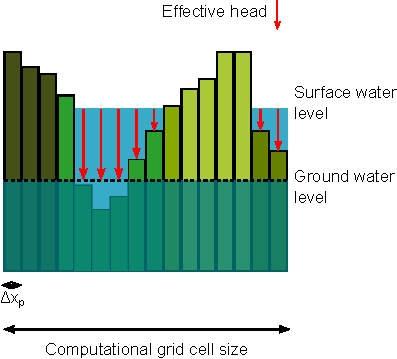
\includegraphics[width=0.48\textwidth]{subgrid_hydrology}
\caption{Subgrid infiltration into heterogeneous landscape.}
\label{fig:figure2}
\end{wrapfigure}

In between these interface calls, the model state may be changed from outside and the core should support that. The library is loaded and can serve as a running process for a long time. A positive side-effect of implementing this interface is that it reveals subtle inconsistencies in existing code, for example initializing different models after one another: incomplete cleanup of previous settings, already allocated memory, unclosed file pointer all become apparent. To reduce the number of errors a template system was introduced to generate the code used to allocate, deallocate, and expose the variables.

The planter size pixel resolution of the digital terrain maps for detailed evaluation of overland flow friction and water storage is described in \citet{Stelling2012}. To represent water systems in civilized regions the 2D grid was extended 1D channels and controllable structures (for example pumps, orifices, weirs). This allows for more realistic and interactive overland flooding simulation.

The power of the subgrid concept is also applied the hydrological processes in the subsoil. An important factor in potential flooding is the storage of water in the subsoil, or the lack thereof. The change in surface water volume is driven by several familiar processes:
\[
\Delta V_\mathrm{surface\ water} = (Q_\mathrm{overland} + Q_\mathrm{precipitation} - Q_\mathrm{infiltration} - Q_\mathrm{evaporation} + Q_\mathrm{drainage})\cdot\Delta t
\]

The heterogeneous landscape and land use are specified in the model as gigapixel bitmaps for soil types, crop types, drainage resistance, and maximum infiltration.  Infiltration, evaporation, and drainage are evaluated at pixel resolution, whereas the computational grid cells are larger and ensure high performance.

These advances in the numerical model allow the model to act as a component in the interactive web-based model environment with a wide variety of possible applications.


\section{Architecture}
Now that a numerical model is available that allows high resolution interactive modeling, how can we hook it up to a tablet, mobile phone and map table, all at the same time, to allow for social and interactive modeling?

To enable such an environment the most logical choice is to use a web-based environment. Over the last years this choice has become more apparent. The large list of browser enhancements (for example inline \ac{SVG}, canvas, plugin free video \citep{Berjon2014}, and \ac{CSS} animations \citep{Jackson2013}) allow for rich visualizations independent of the device type. An overview of the system architecture is given in \autoref{fig:arch}. The architecture follows the general ``Model View Controller'' pattern \citep{Gamma1994}, with caching of events and data to accommodate for the model continuously running in the background. The implementation of this system required several technical innovations and social considerations.

\begin{wrapfigure}[9]{r}{0.5\textwidth}
  \centering
  \vspace{-20pt}
  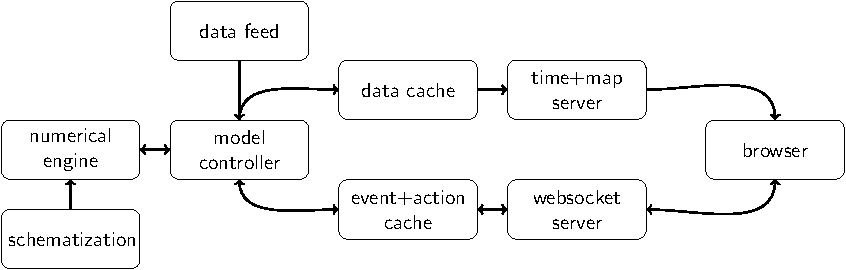
\includegraphics[width=0.48\textwidth]{arch}
  \caption{Architecture overview}
  \label{fig:arch}
\end{wrapfigure}

The end-users, interact with the web-based \ac{GUI}. The design philosophy is minimalistic, allowing little room for user mistakes. For example discharge locations only have two options (normal and extreme discharge) (see \autoref{fig:twod}). Sessions with groups of end-users resulted in this design that provides freedom to explore without the insinuation that the model results are ``true''.

One of the differences when comparing a desktop user to a web-based user is the short attention span. If no indication of progress is given for longer than two second users will start reloading, clicking erratically or will just close the website, searching for a new ``frisson'' \citep{Carr2011}. To make sure that the model is ready to run when a user arrives a lot of attention is given to the provisioning of the model. Provisioning, in this context, is preparing a model controller so that it starts its computation on request. Machines are prepared and put on hold at one of the \ac{IaaS} providers (such as Amazon). These machines are prepared with a container that contains the model schematization, tables and grids, and hot restart files. These files are read into memory so that the model is ready to start its computation when needed, resulting in a time between a user logging in and a model start in under 5 seconds.

To communicate the model results the \ac{MMI} protocol is used \citep{Baart2014a}. This protocol is suitable for sending model variables over the internet. A model message consists of a metadata header in \ac{JSON} format, optionally followed by bytes. Listing \ref{lst:mmi} shows an example of an \ac{MMI} message. In this project the \ac{0MQ} protocol is used as a the underlying transport protocol. The advantage of using the \ac{MMI}, \ac{0MQ} combination is that it has flexible metadata, does not copy data is very fast.

\begin{lstlisting}[caption=MMI message,label=lst:mmi]
# The first part of the message contains metadata
{
  "name": "waterlevel",
  "shape": [3,3],
  "dtype": "float64",
  "attributes": {
       "standard_name": "sea_surface_altiude",
       "units": "m"
  }
}
# The second part of the message contains bytes
\x81\xb3b\xa0\xe8 ... \x01\x90\xe5\x84\xb5\xb0
\end{lstlisting}

Interaction is another challenge where timing is crucial. When a user interacts with the model, for example places a discharge point, turns on a pump or lowers an orifice, the user expects a response within a second. This short feedback loop is achieved using several techniques. User interactions are directly send through websockets \citep{Hickson2012} to the model controller. These interactions are cached and pushed into the model on every timestep. These timesteps have to be kept shorter than in a classical model run, \SI{100}{\milli\second} is common. After a model timestep the chain is inverted. The model pushes it's arrays back in the direction of the browser, which is subscribed to these messages and can directly visualize the results. This fast feedback loop gives a good sense of interactivity.

The social aspect of modeling is another aspect where interesting problems occur. Several group sessions with different settings have been tried. The current setup is that the model is run in a ``virtual room'', like a chat room. Multiple people can join the model run. One person is in control and others can view and zoom in on the same model run. Other users can request control of the model. The sessions worked best when a topic expert, not necessary a modeler, was present in the session.

\section{Visualization}
The \threedi platform serves a wide variety of end-users. It is important to find a good balance between what is computed and how information is perceived. For scientific or engineering users one wants to provide information as close to the model results as possible. For less experienced end users it becomes important that the information is perceived correctly rather than that it is presented correctly.

First a note about the performance. Humans will detect images at a rate of about \SI{12}{\per\second} as continuous \citep{Landis1954}. To enable the model results to be perceived as continuous, taking into account some random network delay, the aim is to generate a map within \SI{50}{\milli\second}. Generating results at this framerate can be done using two approaches. The first is to reduce the timestep so that it computes in less than \SI{50}{\milli\second}. This is the only way to get true model results at this framerate. An alternative is to interpolate in time and provide the insinuation of continuous information. We use both approaches here. We reduce the calculation time so that interaction is fluent and we can pass the flicker fusion threshold. If one wants to use longer time steps we also visualize at a high framerate. An example of this is the visualization of river flow using dots that are animated with \ac{CSS} animations as a function of the current flow velocity (see \autoref{fig:oned}).

Another performance technique used to achieve the high framerate is to use the ``Mahlen nach Zahlen'' method, a reference to a product from the German company Ravensburger~\textregistered. A map with cell numbers is prepared in advance. Once a quantity for a new timestep becomes available the map is filled in with the colors corresponding to the cell numbers. This achieves much faster rendering times than drawing the cells using geometry drawing function.

\begin{figure}[htbp]
  \centering

  \begin{subfigure}{0.4\textwidth}
    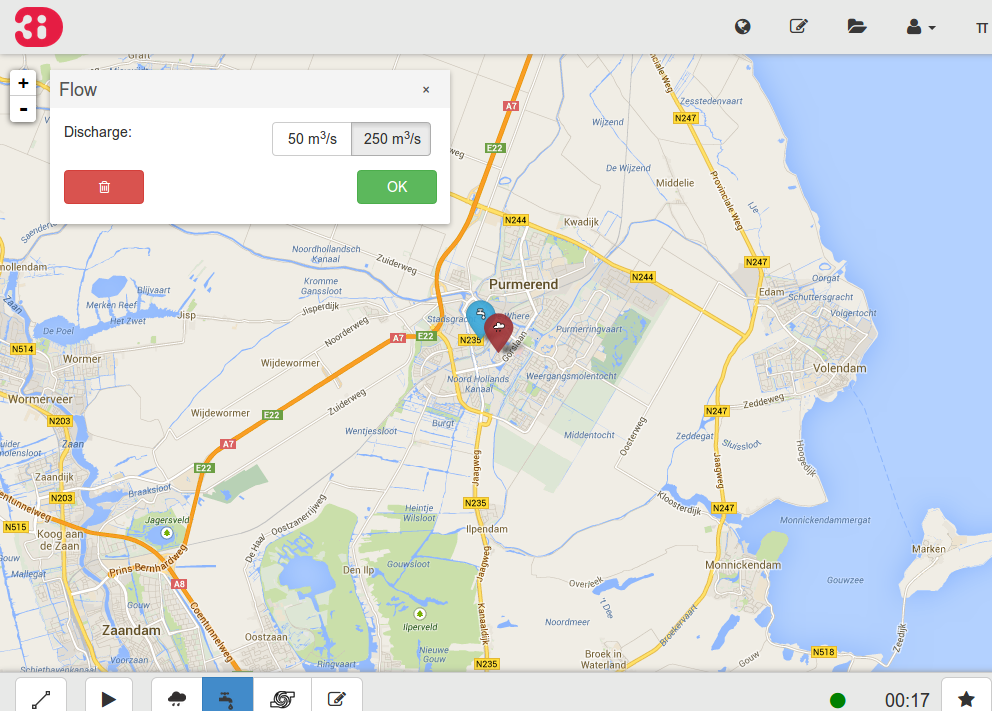
\includegraphics[width=1\textwidth]{webgui}
    \caption{Representation of two dimensional subpixels water level}
    \label{fig:twod}
  \end{subfigure}
  \begin{subfigure}{0.4\textwidth}
    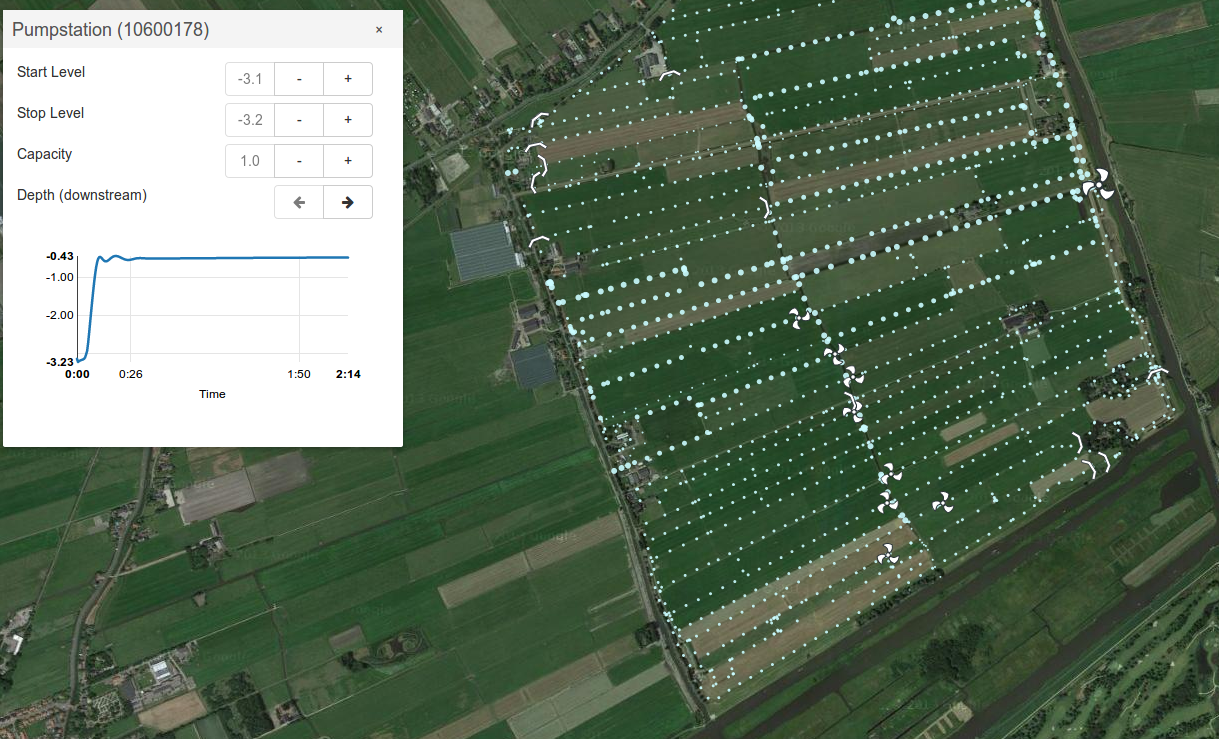
\includegraphics[width=1\textwidth]{oned}

    \caption{Representation of one dimensional channel network using an animated stroke pattern.}
    \label{fig:oned}
  \end{subfigure}
  \label{fig:gui}
  \caption{Browser based interactive model user interface of \threedi}
\end{figure}

The variety of end-users exposes the numerical model to non-technical users with little appreciation of implemented numerical schemes. Some artifacts from the numerical schemes result in confusion. The world in the subgrid model is internally represented in voxels, not unlike the computer game Minecraft. This results in visual artifacts, as represented in \autoref{fig:arta}. Another type of artifact occurs when a levee crosses a calculation cell both sides of the cell will contain water.

One can argue whether to show these ``true'' yet confusing results or to process the information so that is perceived as intended. In the \threedi platform the default visualization hides these artifacts by filtering and smoothing the output. Hiding the square world is implemented using different techniques.

\begin{figure}[htpb]
  \centering
  \begin{subfigure}{0.4\textwidth}
    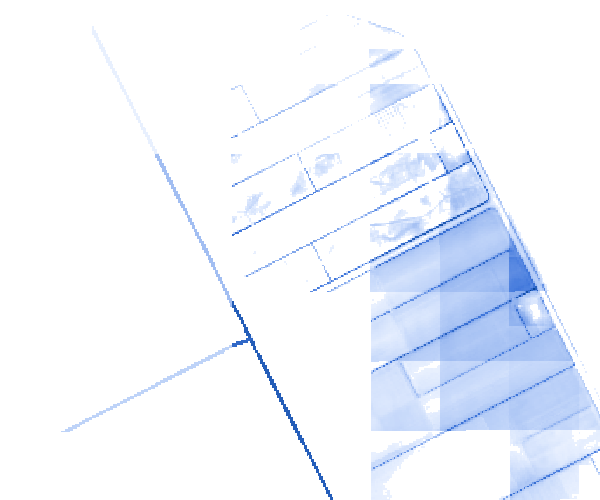
\includegraphics[width=1\textwidth]{arta}
    \caption{Uninterpolated subgrid water level}
    \label{fig:arta}
  \end{subfigure}
  \begin{subfigure}{0.4\textwidth}
    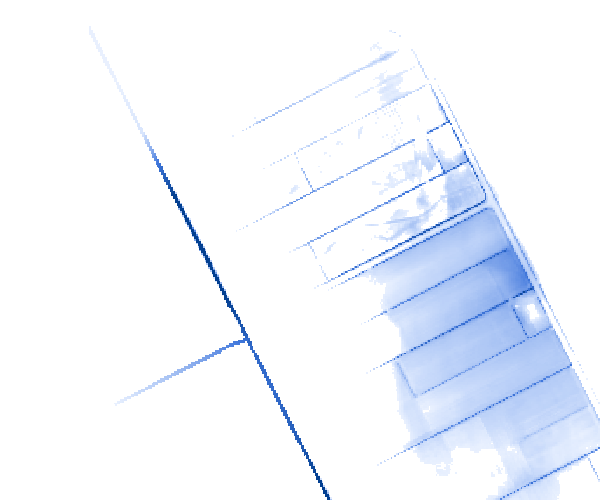
\includegraphics[width=1\textwidth]{artb}
    \caption{Interpolated subgrid water level}
    \label{fig:artb}
  \end{subfigure}
  \label{fig:artifacts}
  \caption{Interpolation method}
\end{figure}

A barycentric linear interpolation technique is used. This is one of the few techniques that allow for the interpolation within the rendering time constraint. It also allows to interpolate water level results on an arbitrary grid. The quad tree grid is triangulated using Qhull \citep{Barber1996}.  Water level information, from the cell centers and is linearly interpolated to the underlying subgrid. The interpolation uses a weighted average the determine water levels. The triangular mesh can be reused.   \autoref{fig:artb} shows the results of this technique .

\begin{figure}[htbp]
  \centering
  \begin{subfigure}{0.4\textwidth}
    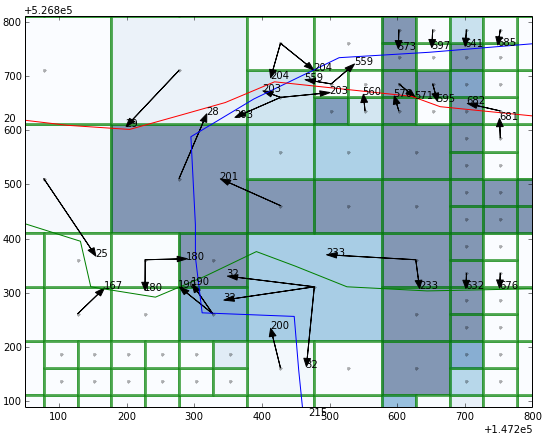
\includegraphics[width=1\textwidth]{levees1}
    \caption{Redistribution of cell sections based on levee positioning.}
    \label{fig:levee1}
  \end{subfigure}
  \begin{subfigure}{0.4\textwidth}
    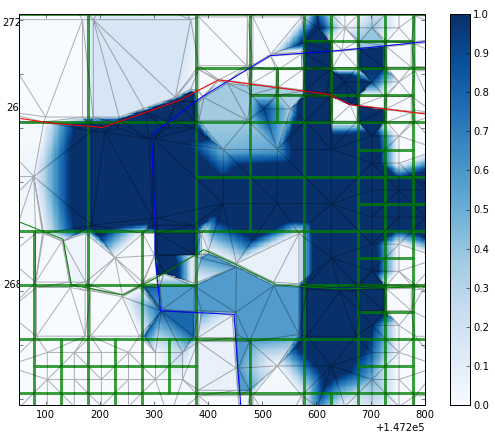
\includegraphics[width=1\textwidth]{levees2}
    \caption{Interpolated subgrid water level with levee constrained}
    \label{fig:levee2}
  \end{subfigure}
  \label{fig:levees}

  \caption{Levee-constrained interpolation method}

\end{figure}

The triangulation within the linear barycentric interpolation also allows us to filter levee artefacts of the numerical model. The calculation grid incorporates the function of a levee in the numerical schemes. However it disregards the actual position of such a levee within a calculation cell. The triangulation can reconstruct levees with use of additional levee geometries. A triangle is one of the simplest geometrical forms and can be used reconstruct any arbitrary shape \citep{Welch1994}. To incorporate the levee in the trianglulation, the levee and grid geometries are intersected (\autoref{fig:levee1}). For the intersected calculation cells the influential water level points are determined and coupled to the relevant calculation areas. The arrows in \autoref{fig:levee1} indicate which water level is relevant for the dike intersected cell areas. When all waterlevel points are allocated to the dike, the triangulation can be executed with the incorporation of the levee geometries. The newly created triangular mesh now also follows the added levee geometry. Successively the interpolation is executed, resulting in water being retained behind the dike within one calculation cell. The interpolated result is shown in \autoref{fig:levee2}.



\section{Discussion and conclusion}
Several other models use a similar numerical approach, albeit with limitations. The subgrid scheme by \citet{Stelling2012} is partly based on the subgrid method for flooding and drying by \citet{Casulli2009}, who implements his methods in the UnTRIM research package \citet{Casulli2000}. UnTRIM uses fully unstructured grids as opposed to the quad tree grids used here. The coupled 1D-2D hydrodynamic model MIKE-FLOOD \citep{Dhi2014} also offers subgrid overland flow. In the accompanying MIKE-SHE all relevant vertical hydrological processes are offered, also with some degree of subgrid-information for the infiltration part.

The major advancement here is to redesign the numerical engine into a component that allows for external control and introspection. By combining this numerical model with the technical advancements described in this paper, we have enabled interactive web-based modeling at a high resolution and wide coverage.

A lot of technical and numerical problems have been solved, but the methodological challenges of the new working methods are proving more difficult. An open issue is that end-users tend to confuse high resolution and higher frequency results with a high accuracy, a topic for further research.

Possible future directions include combining the subgrid approach with an unstructured flow solver, such as Delft3D-FLOW Flexible Mesh \citep{Kernkamp2011}. The pixel based approach has the advantage that it is simple to implement and to scale. Unfortunately the world is not so square, especially not on larger scales, when one goes beyond the scale of a small country.

Another planned step is to incorporate or preferably to couple the system with other physical models. The monolithic approach of putting all processes into one model has proven cumbersome in previous implementations. The current model controller can easily incorporate other models because the communication and control are already out of the model engine. Water quality, coastal, and socio-economic models are possible candidates for inclusion in the platform.

Viewing model results through the web is already a reality (see \citep{Blower2013} for example). We have made progress to run and interact with models through the browser. What is not available, for complex models, is the ability to set up a new model through the web. At the moment it is still cumbersome to implement this functionality. However within the next few years it is likely that also this part of the modeling workflow will become browser-based.

%%%%%%%%%%%%%%%%%%%%%%%%%%%%%%%%%%%%%%%%%%%%%%%%%%%%%%%%%%%%%%%%%
\bibliographystyle{apalike}
\bibliography{./bibliography}
%%%%%%%%%%%%%%%%%%%%%%%%%%%%%%%%%%%%%%%%%%%%%%%%%%%%%%%%%%%%%%%%%
\begin{acronym}[AAAAA]
\acro{CSS}{Cascading Style Sheets}
\acro{MMI}{Model Message Interface}
\acro{JSON}{JavaScript Object Notation}
\acro{0MQ}[\O{}MQ]{Zero Message Queue}
\acro{SVG}{Scalable Vector Graphics}
\acro{H2O}[$\mathrm{H_2O}$]{water}
\acro{BMI}{Basic Model Interface}
\acro{API}{Application Programming Interface}
\acro{GUI}{Graphical User Interface}
\acro{DEM}{Digital Elevation Model}
\acro{HTTP}{Hyper Text Transfer Protocol}
\acro{IaaS}{Infrastructure as a Service}
\end{acronym}



\end{document}
